\chapter{测试与实验}

\section{测试总述}
本章节包含了对本文所带的样例实现进行简单测试的过程和结果。测试主要通过对客户端库进行数个集成的测试,而服务端不包含单独的测试。对服务端的测试被包含在对客户端库的测试中,通过对网络通信函数的测试来间接完成。对每个测试本章节亦会给出其对应的基准测试结果。

\section{测试环境描述}

\subsection{系统环境}

\begin{itemize}
    \item 操作系统:Arch Linux(Rolling)\footnote{即滚动性发行,所有软件包总是上游最新的}
    \item Golang 工具链:版本 1.20.4,Arch 软件包仓库版本 \verb|go 2:1.20.4-1|
    \item 处理器:AMD Ryzen 9 4900HS with Radeon Graphics (16) @ 3.000GHz
\end{itemize}

\subsection{样例实现使用的第三方库}

以下为本方案所使用的第三方库列表。其中,\verb|github.com/tuneinsight/lattigo/v4| 为本方案的核心库,其余为辅助库。

\begin{minted}{go}
require (
    github.com/tuneinsight/lattigo/v4 v4.1.0
    github.com/urfave/cli/v2 v2.25.1

    github.com/google/uuid v1.3.0
    github.com/kr/pretty v0.3.1
    github.com/mattn/go-sqlite3 v1.14.16
    github.com/pkg/errors v0.9.1
)
\end{minted}

\section{测试样例描述}

本方案编写了如下测试函数,其中每个测试函数都有对应的性能基准测试函数:

\begin{itemize}
    \item \verb|func TestCKKSEncryptAndDecrypt(*testing.T)|:对本文代码封装的 CKKS 加密和解密函数进行正确性测试;
    \item \verb|func TestTransferBySenderPK(*testing.T)|:测试能否正确生成交易;
    \item \verb|func TestTransferByReceiptPK(*testing.T)|:同上;
    \item \verb|func TestAcceptTransactionByTransaction(*testing.T)|:测试能否正确生成确认消息;
    \item \verb|func TestRegisterUser(*testing.T)|:测试生成密钥对,将用户信息提交给服务端的功能,并且测试服务端是否能够正确地将用户信息存储到数据库中而不报出异常;
    \item \verb|func TestRegisterSwk(*testing.T)|:在上述函数基础上,测试生成交换密钥,并将其提交给服务端;
    \item \verb|func TestCreateTransferJob(*testing.T)|:在上述函数基础上,测试能否正确向服务端提交交易信息,以及服务端是否会正确响应请求;
\end{itemize}

以及以下的辅助函数:

\begin{itemize}
    \item \verb|func initTestRandomUser()|:准备单次测试环境,包括全局变量等。
    \item \verb|func makeNewRandomUser(string)|:生成随机用户。
\end{itemize}

\section{实验和基准测试结果}

本文在测试时,使用下述命令,调用 Golang 工具链提供测试功能,对方案进行功能测试和性能测试。

\begin{minted}{shell}
$ go run ./cmd/server # 使服务端上线

# 进行集成测试
$ /usr/bin/go test -timeout 30s \
  -coverprofile=/tmp/vscode-goUzLyPD/go-code-cover \
  github.com/CamberLoid/Chimata/internal/clientlib

# 进行基准性能测试
$ /usr/bin/go test -benchmem -run=^$ \
  -coverprofile=/tmp/vscode-goUzLyPD/go-code-cover \
  -bench . github.com/CamberLoid/Chimata/internal/clientlib
\end{minted}

测试结果如下图\ref*{Fig:test} \ref*{Fig:benchmark} \ref*{Fig:server}所示。

\begin{figure}[ht]
    \centering
    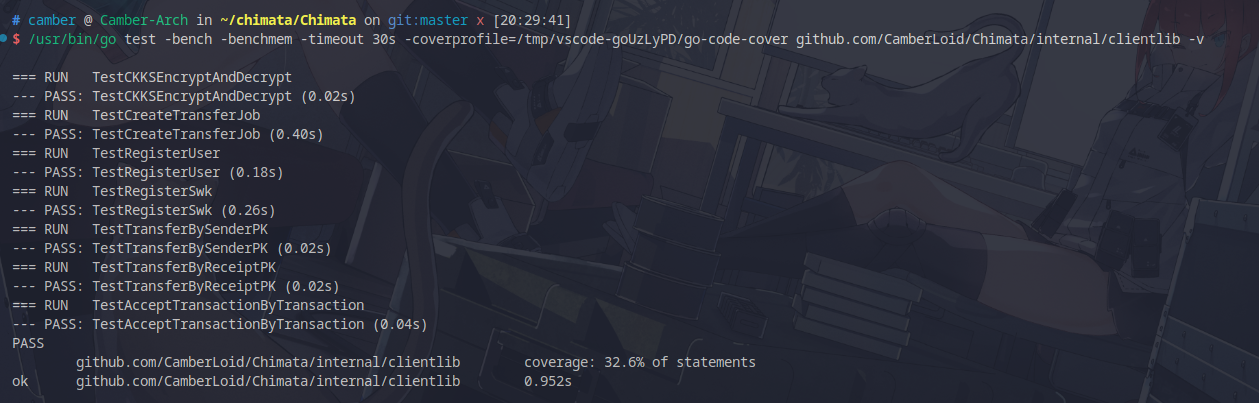
\includegraphics[width=0.8\linewidth]{./Figures/Test.png}
    \caption{集成测试输出}\label{Fig:test}
\end{figure}

\begin{figure}[ht]
    \centering
    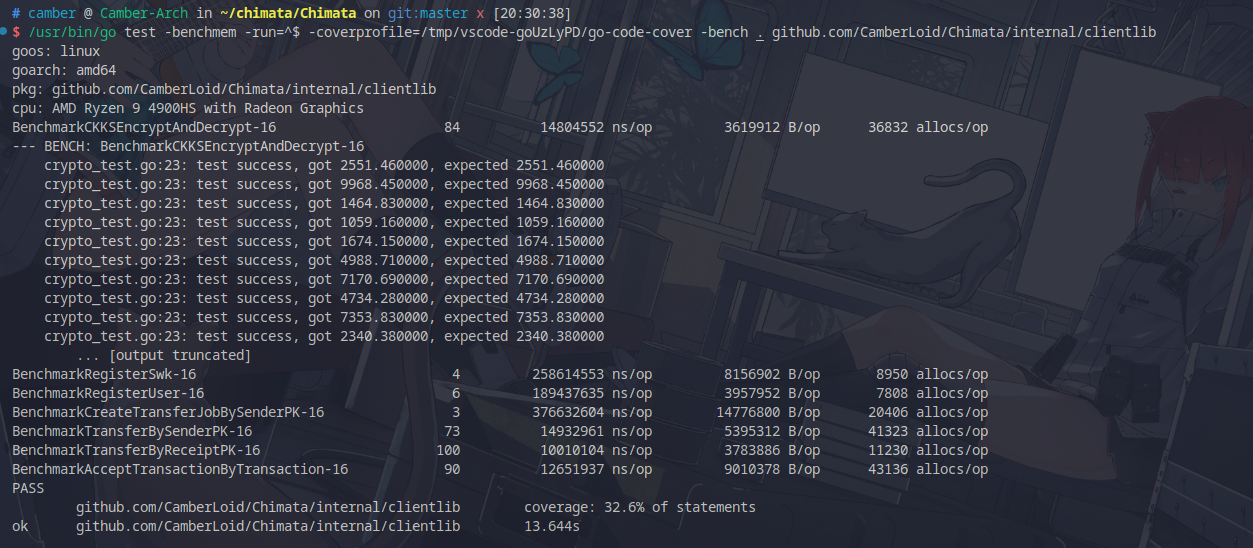
\includegraphics[width=0.8\linewidth]{./Figures/Benchmark.png}
    \caption{性能测试输出}\label{Fig:benchmark}
\end{figure}

\begin{figure}[ht]
    \centering
    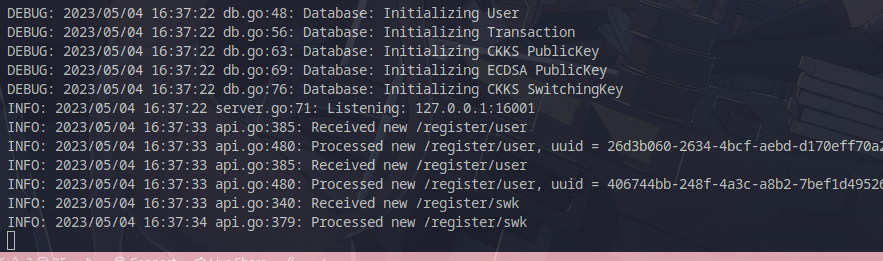
\includegraphics[width=0.8\linewidth]{./Figures/Server.png}
    \caption{服务端日志输出}\label{Fig:server}
\end{figure}
